\documentclass[review]{elsarticle}

% to remove elsearticle 'preprint journal'
\makeatletter
\def\ps@pprintTitle{%
 \let\@oddhead\@empty
 \let\@evenhead\@empty
 \def\@oddfoot{\centerline{\thepage}}%
 \let\@evenfoot\@oddfoot}
\makeatother
%%\journal{IB200}

\usepackage[hidelinks]{hyperref}
\usepackage{mathtools}
\usepackage{adjustbox}
\usepackage{natbib}
\usepackage{booktabs}
\usepackage{lineno}

\graphicspath{ {./figures/} }

%% bibliography styles
%% Harvard
\bibliographystyle{model2-names}\biboptions{authoryear}
%% `Elsevier LaTeX' style
%\bibliographystyle{elsarticle-num}



%%%%%%%%%%%%%%%%%%%%%%%
%% front matter
%%%%%%%%%%%%%%%%%%%%%%%

\begin{document}

\begin{frontmatter}

\title{Patterns of floral and chromosome evolution in Onagraceae: a fossil-calibrated supermatrix analysis}

\author[berk]{William A. Freyman\corref{cor1}}
\ead{freyman@berkeley.edu}
\cortext[cor1]{Corresponding author}

\address[berk]{Jepson Herbarium and Department of Integrative Biology, University of California, Berkeley}

\begin{abstract}
Onagraceae is a cosmopolitan plant family in the order Myrtales comprised of 22 genera and 657 species.
I used a GenBank data-mining approach to construct an 11 gene supermatrix of 521 taxa in Onagraceae and Lythraceae.
Maximum likelihood and Bayesian inference phylogenetic analyses were performed, 
and divergence time estimates were calibrated using 5 fossils.
Chromosome number evolution was inferred using probabilistic models,
and ancestral states of petal color and petal number were reconstructed using maximum likelihood.
Correlated evolution between petal color and petal number was tested using
Bayesian stochastic character mapping.
The monophyly of all major clades in Onagraceae was supported,
and Onagraceae was estimated to have diverged from Lythraceae 109 Mya. 
The base chromosome number of Onagraceae was inferred to be $x=5$.
Petal color and petal number were found
to follow a pattern of correlated evolution ($p=0.00$), 
suggesting concerted shifts in floral traits may play an important role in shaping diversification of Onagraceae. 
Further analyses should be performed to test whether shifts in
floral traits are correlated with pollinator shifts,
and to determine how these shifts affect diversification rates.
Furthermore, this work should be extended to test historical biogeographical hypotheses
that explain the intercontinental disjunct distribution of Onagraceae.
\end{abstract}

\end{frontmatter}


%%%%%%%%%%%%%%%%%%%%%%%
%% intro
%%%%%%%%%%%%%%%%%%%%%%%

%\modulolinenumbers[5]
%\linenumbers

\section{Introduction}

Introduce supermatrix analyses....

Onagraceae, the evening primroses, are a well-studied family
of flowering plants with 22 described genera and around 660 species \citep{wagner2007revised}.
The family is found on all continents except Antartica,
and pollen fossils date Onagraceae to the Upper Cretaceous \citep{grimsson}.
Onagraceae is well placed in the order Myrtales,
and previous molecular phylogenetic studies find it most closely related to Lythraceae \citep{conti1997, Sytsma2004}.
Though there have been many genus-level molecular phylogenetic studies in Onagraceae
\citep{Berry2004, Evans2009, Hoggard2004, Xie2009, Baum1994, Wagner2005}, 
the most recent family-level analyses \citep{Levin2003, Levin2004}
used only one or two exemplars from some genera. 
Furthermore, the historical biogeography, divergence times of the major clades, and 
family-level patterns and processes of diversification remain poorly understood.
With the wealth of data available, Onagraceae is an
ideal group to apply a data-mining supermatrix approach
with the goal of constructing a densely sampled family-level phylogeny.

Here, I use a well-resolved supermatrix phylogeny of Onagraceaea to
answer qestions such as:
1) Are the taxonomic groups described in \citet{wagner2007revised} monophyletic?
2) When did the major clades diverge?
3) What is the pattern of chromosome number
evolution?
4) What are the patterns of petal color and petal number evolution, and are their 
evolution correlated?
Finally, I also discuss ways in which these analyses can be extended
to further examine the patterns and processes of
evolution in Onagraceae.


\section{Methods}

\paragraph{Supermatrix assembly} 

Lythraceae was selected as an outgroup since previous molecular phylogenetic analyses
place it sister to Onagraceae \citep{conti1997, Sytsma2004}.
I downloaded all DNA sequences from GenBank release 200 PLN division and
performed an exhaustive all-by-all BLASTn \citep{blast} comparison of sequences in Onagraceae
and Lythraceae.
Using a BLASTn e-value of $1.0 \times 10^{-10}$ threshold and a sequence length
percent similarity cutoff of 0.5,
I constructed clusters of putative homologs using a single-linkage hierarchical clustering algorithm.
Subspecies names were removed from all sequences, and all but one sequence of each species was pruned from each cluster.
Clusters that were not phylogenetically informative ($< 4$ taxa) were discarded,
and each cluster was aligned using MUSCLE \citep{edgar2004muscle}. 
The alignments were concatenated by species, and any species that was not present in at least
two clusters was removed from the supermatrix.
The program written to data-mine GenBank and assemble the supermatrix 
is available as the open source Python module 
SUMAC \citep{sumac}.
SUMAC will assemble
supermatrices for any taxonomic group recognized in GenBank, 
and is optimized to run on multicore processors and clusters by utilizing multiple parallel processes.



\paragraph{Phylogenetic analyses} 
Maximum likelihood (ML) analyses were performed with RAxML-HPC \citep{raxml} on the CIPRES Scientific Gateway \citep{cipres} 
using the rapid bootstrap heuristic and the GTRCAT nucleotide substitution model.
I used the ML tree to select 15 taxa phylogenetically widely distributed in Lythraceae to act as outgroup for the divergence time analysis; 
all other members of Lythraceae were subsequently removed from the supermatrix.
Bayesian estimates of divergence times were inferred using BEAST v1.8 \citep{beast, beast2} on CIPRES and calibrated with five fossils 
identified with morphological synapomorphies (Table \ref{fossils}).
The \textit{Ludwigia} fossil pollen was dated broadly to the Paleocene \citep{grimsson}, so I set the prior to a normal distribution with a wide 
standard deviation to cover the entire time period.
For all other calibration points I used a lognormal prior distribution with the offset (the minimum age of the node) corresponding to the fossil age.
The BEAST analysis utilized the GTR+$\Gamma$ nucleotide substitution model with a relaxed molecular clock (uncorrelated lognormal model)
and a Yule process tree prior.
The Markov Chain Monte Carlo (MCMC) was run for 100 million generations, sampling every 10 thousand generations.
Tracer v1.6 \citep{tracer} was used to assess the MCMC output for parameter convergence and ensure that the effective sample size for all parameters was above 200.
The first 1000 trees were discarded as burn-in, and the remaining 9000 trees were summarized as a maximum clade credibility (MCC) tree with mean divergence times. 

\begin{table*}
   \center
   \begin{adjustbox}{max width=\textwidth}
      \begin{tabular}{lllllll}
         \toprule
         Group & Age (Mya) & Prior Distribution & Mean & SD & Offset & Reference \\ 
	 \midrule
         \textit{Circaea} (Onagraceae) & 12 & lognormal & 0.0 & 2.0 & 12 & \citep{grimsson} \\
         \textit{Epilobium} (Onagraceae) & 12 & lognormal & 0.0 & 2.0 & 12 & \citep{grimsson} \\
         S. Pacific \textit{Fuschia} (Onagraceae) & 23 & lognormal & 0.0 & 1.0 & 23 & \citep{lee2013fossil} \\
         \textit{Ludwigia} (Onagraceae) & Paleocene & normal & 60.0 & 3.0 & - & \citep{zhi} \\
         Lythraceae & 82 & lognormal & 0.0 & 2.0 & 82 & \citep{graham} \\
         \bottomrule
      \end{tabular}
   \end{adjustbox}
   \caption{Fossils used as priors in the Bayesian divergence time analysis.}
   \label{fossils}
\end{table*}

\paragraph{Character state reconstruction}
I scored six characters, including
chromosome number, floral merosity, petal color, and self-compatibility/incompatibility. 
Character data was assembled from the comprehensive \citet{wagner2007revised} Onagraceae monograph.
Ancestral chromosome numbers were inferred using maximum likelihood and Bayesian methods 
as implemented in ChromEvol 2.0 \citep{chromevol}.
Eight different models of chromosome evolution were fit to the Bayesian MCC phylogeny using ChromEvol,
and the best fit model was selected using Akaike's information criterion \citep{aic}.
Ancestral character state reconstructions of petal number and petal color were performed using Mesquite v2.75 \citep{mesquite}
over the Bayesian MCC tree.
Characters were treated as unordered categorical data, and optimized using maximum likelihood
with the Markov k-state 1 parameter (Mk1) model \citep{lewis2001likelihood}.
Additionally, Bayesian stochastic character mapping \citep{Huelsenbeck2003} was used to test whether
petal color and petal number covaried over the phylogeny. 
Models of petal color and petal number evolution
were configured in the program SIMMAP v1.5 \citep{bollback2006simmap}
using unordered states, gamma rate priors, and equal state bias priors.
The correlation analysis used SIMMAP's default
predictive sampling configuration
and calculated the following correlation statistics: 
$D$ the overall association between
the two characters, and $d_{ij}$ the association between the
individual states of each character \citep{Huelsenbeck2003}.


%%%%%%%%%%%%%%%%%%%%%%%
%% results
%%%%%%%%%%%%%%%%%%%%%%%

\section{Results}


\paragraph{Supermatrix assembly}
SUMAC evaluated 5571 Onagraceae and 2832 Lythraceae nucleotide sequences to construct the supermatrix. 
The completed supermatrix consisted of 11 clusters of homologous sequences (Table \ref{clusters}).
As used in the maximum likelihood analyses (before pruning the number of outgroup taxa), 
the supermatrix contained 521 taxa, was 31862 nucleotides long, and contained 93.0\% missing data.

\begin{table*}
   \center
   \begin{adjustbox}{max width=\textwidth}
      \begin{tabular}{lllllll}
         \toprule
         DNA Region & \# of Taxa & Aligned Length & Missing data (\%) & Taxon Coverage Density \\ 
	 \midrule
         ITS & 453 & 1746 & 13.2 & 0.87 \\
         trnL & 234 & 1429 & 55.2 & 0.45 \\
         rpl16 & 91 & 1414 & 82.6 & 0.17 \\
         rbcL & 77 & 1474 & 85.2 & 0.15 \\
         rps16 & 74 & 1016 & 85.8 & 0.14 \\
         rbcL2 & 64 & 1310 & 87.7 & 0.12 \\
         PgiC2 & 47 & 4028 & 91.0 & 0.09 \\
         matK & 37 & 921 & 92.9 & 0.07 \\
         ndhF & 37 & 2063 & 92.9 & 0.07 \\
         pgiC & 26 & 14709 & 95.0 & 0.05 \\
         R5 & 18 & 3129 & 96.6 & 0.03 \\
         \bottomrule
      \end{tabular}
   \end{adjustbox}
   \caption{Clusters of homologous sequences used to assemble the supermatrix.}
   \label{clusters}
\end{table*}

\paragraph{Phylogeny and divergence time estimates}
The topologies of the ML and Bayesian phylogenies were nearly identical for all major clades within Onagraceae, 
so only the Bayesian MCC tree (Figures \ref{posteriors} and \ref{genera}) is shown here.
The major exception is that in the ML tree the genus \textit{Chamerion} was recovered
as sister to \textit{Epilobium}, whereas in the MCC tree XXXXXX.......
In the MCC tree all Onagraceae genera described in \citet{wagner2007revised} were recovered as monophyletic clades with posterior probabilities $> 0.95$
except for sister genera \textit{Neoholmgrenia} and \textit{Camissoniopsis} (posterior = 0.31) (Figure \ref{posteriors}).
Onagraceae was found to diverge from Lythraceae at 109 Mya (Figure \ref{genera}). 
Divergence time estimates of other major clades and 95\% highest posterior density (HPD) intervals can be seen in Table \ref{times}.

\begin{table*}
   \center
   \begin{adjustbox}{max width=\textwidth}
      \begin{tabular}{lllllll}
         \toprule
         Clade & Mean Age (Mya) & 95\% HPD Min & 95\% HPD Max \\ 
	 \midrule
         Onagraceae / Lythraceae & 109 & 88 & 131 \\
         \textit{Ludwigia} & 97 & 76 & 118 \\
	 \textit{Hauya} & 49 & 35 & 64 \\
	 \textit{Circaea} / \textit{Fuchshia} & 37 & 28 & 47 \\
	 \textit{Lopezia} & 71 & 55 & 68 \\
	 \textit{Gongylocarpus} & 60 & 45 & 77 \\
	 \textit{Epilobium} & 49 & 38 & 60 \\
	 \textit{Chamerion} & 47 & 36 & 57 \\
	 \textit{Xylonagra} & 43 & 33 & 52 \\
	 \textit{Clarkia} & 40 & 32 & 48 \\
         \textit{Terapteron} & 19 & 10 & 29 \\
	 \textit{Camissoniopsis} / \textit{Neoholmgrenia} & 14 & 5 & 23 \\
	 \textit{Eremothera} / \textit{Camissonia} & 24 & 16 & 33 \\
	 \textit{Taraxia} & 30 & 22 & 38 \\
	 \textit{Chylismiella} / \textit{Gayophytum} & 20 & 10 & 30 \\
	 \textit{Eulobus} & 26 & 19 & 34 \\
	 \textit{Chylismia} / \textit{Oenothera} & 25 & 18 & 31 \\
         \bottomrule
      \end{tabular}
   \end{adjustbox}
   \caption{Bayesian divergence time estimates of major clades.}
   \label{times}
\end{table*}

\paragraph{Chromosome number evolution}
Out of the eight models of chromosome evolution tested by ChromEvol,
the four parameter $CONST\_RATE\_DEMI\_EST$ model was the best fit according to the AIC scores. 
This model has separate rate parameters for
chromosome gains ($\lambda$),
losses ($\delta$),
demi-polyploid events ($\mu$),
and polyploid events ($\rho$).
Demi-polyploid events occur when reduced and unreduced gametes unite
resulting in a $3x$ cytotype.
The base chromosome number of Onagraceae was estimated to be $x=5$,
and the ancestral number of the large genus \textit{Epilobium} was estimated to be $n=9$,
though the extant taxa are split in two large monophyletic clades of 
$n=10$ and $n=18$, respectively (Figure \ref{chromtree}).

\paragraph{Floral evolution}
The maximum likelihood estimate of petal color for the 
last common ancestor of Onagraceae was pink 
with a proportional likelihood ($PL$) of $0.56$ (Figure \ref{petal_color}).
White was the second most likely estimate ($PL=0.19$).
The maximum likelihood estimate of petal number for the
last common ancestor of Onagraceae was 4 ($PL=1.0$), with 8
independent transitions to 0, 2, or 5 petals (Figure \ref{petal_number}).
Petal color and petal number were found to significantly covary over the 
phylogeny ($D=0.263, p=0.00$). Multiple signficant correlations
($d_{ij}$) were found between individual states of each character
and are summarized in Table \ref{correlations}.

\begin{table*}
   \center
   \begin{adjustbox}{max width=\textwidth}
      \setlength{\tabcolsep}{20pt}
      \begin{tabular}{llllll}
         \toprule
	 & \multicolumn{3}{c}{Number of Petals} \\
         & 2 & 4 & 5 \\ 
	 \cmidrule{2-4}
	 Petal Color \\
         \hspace{3 mm} Pink & -0.005 & .011 & $ns$ \\
	 \hspace{3 mm} Yellow & -0.008 & .021 & $ns$ \\
	 \hspace{3 mm} White & 0.008 & 0.013 & -0.006 \\
	 \hspace{3 mm} Green & $ns$ & -0.011 & $ns$ \\
	 \hspace{3 mm} Red & $ns$ & $ns$ & $ns$ \\
         \bottomrule
      \end{tabular}
   \end{adjustbox}
   \caption{Test statistics for the correlation between petal color evolution and petal number evolution. 
	    $d_{ij}$ values are shown
            for the pairwise comparison of states with $p< 0.01$. $ns$ indicates no significant
	    association. Negative $d_{ij}$ values express negative correlation.
	    The overall $D$ value was 0.263 ($p=0.00$).
	    }
   \label{correlations}
\end{table*}

\begin{figure*}[p]
    \vspace*{-2cm}
    \makebox[\linewidth]{
        % have to trim bottom off image
        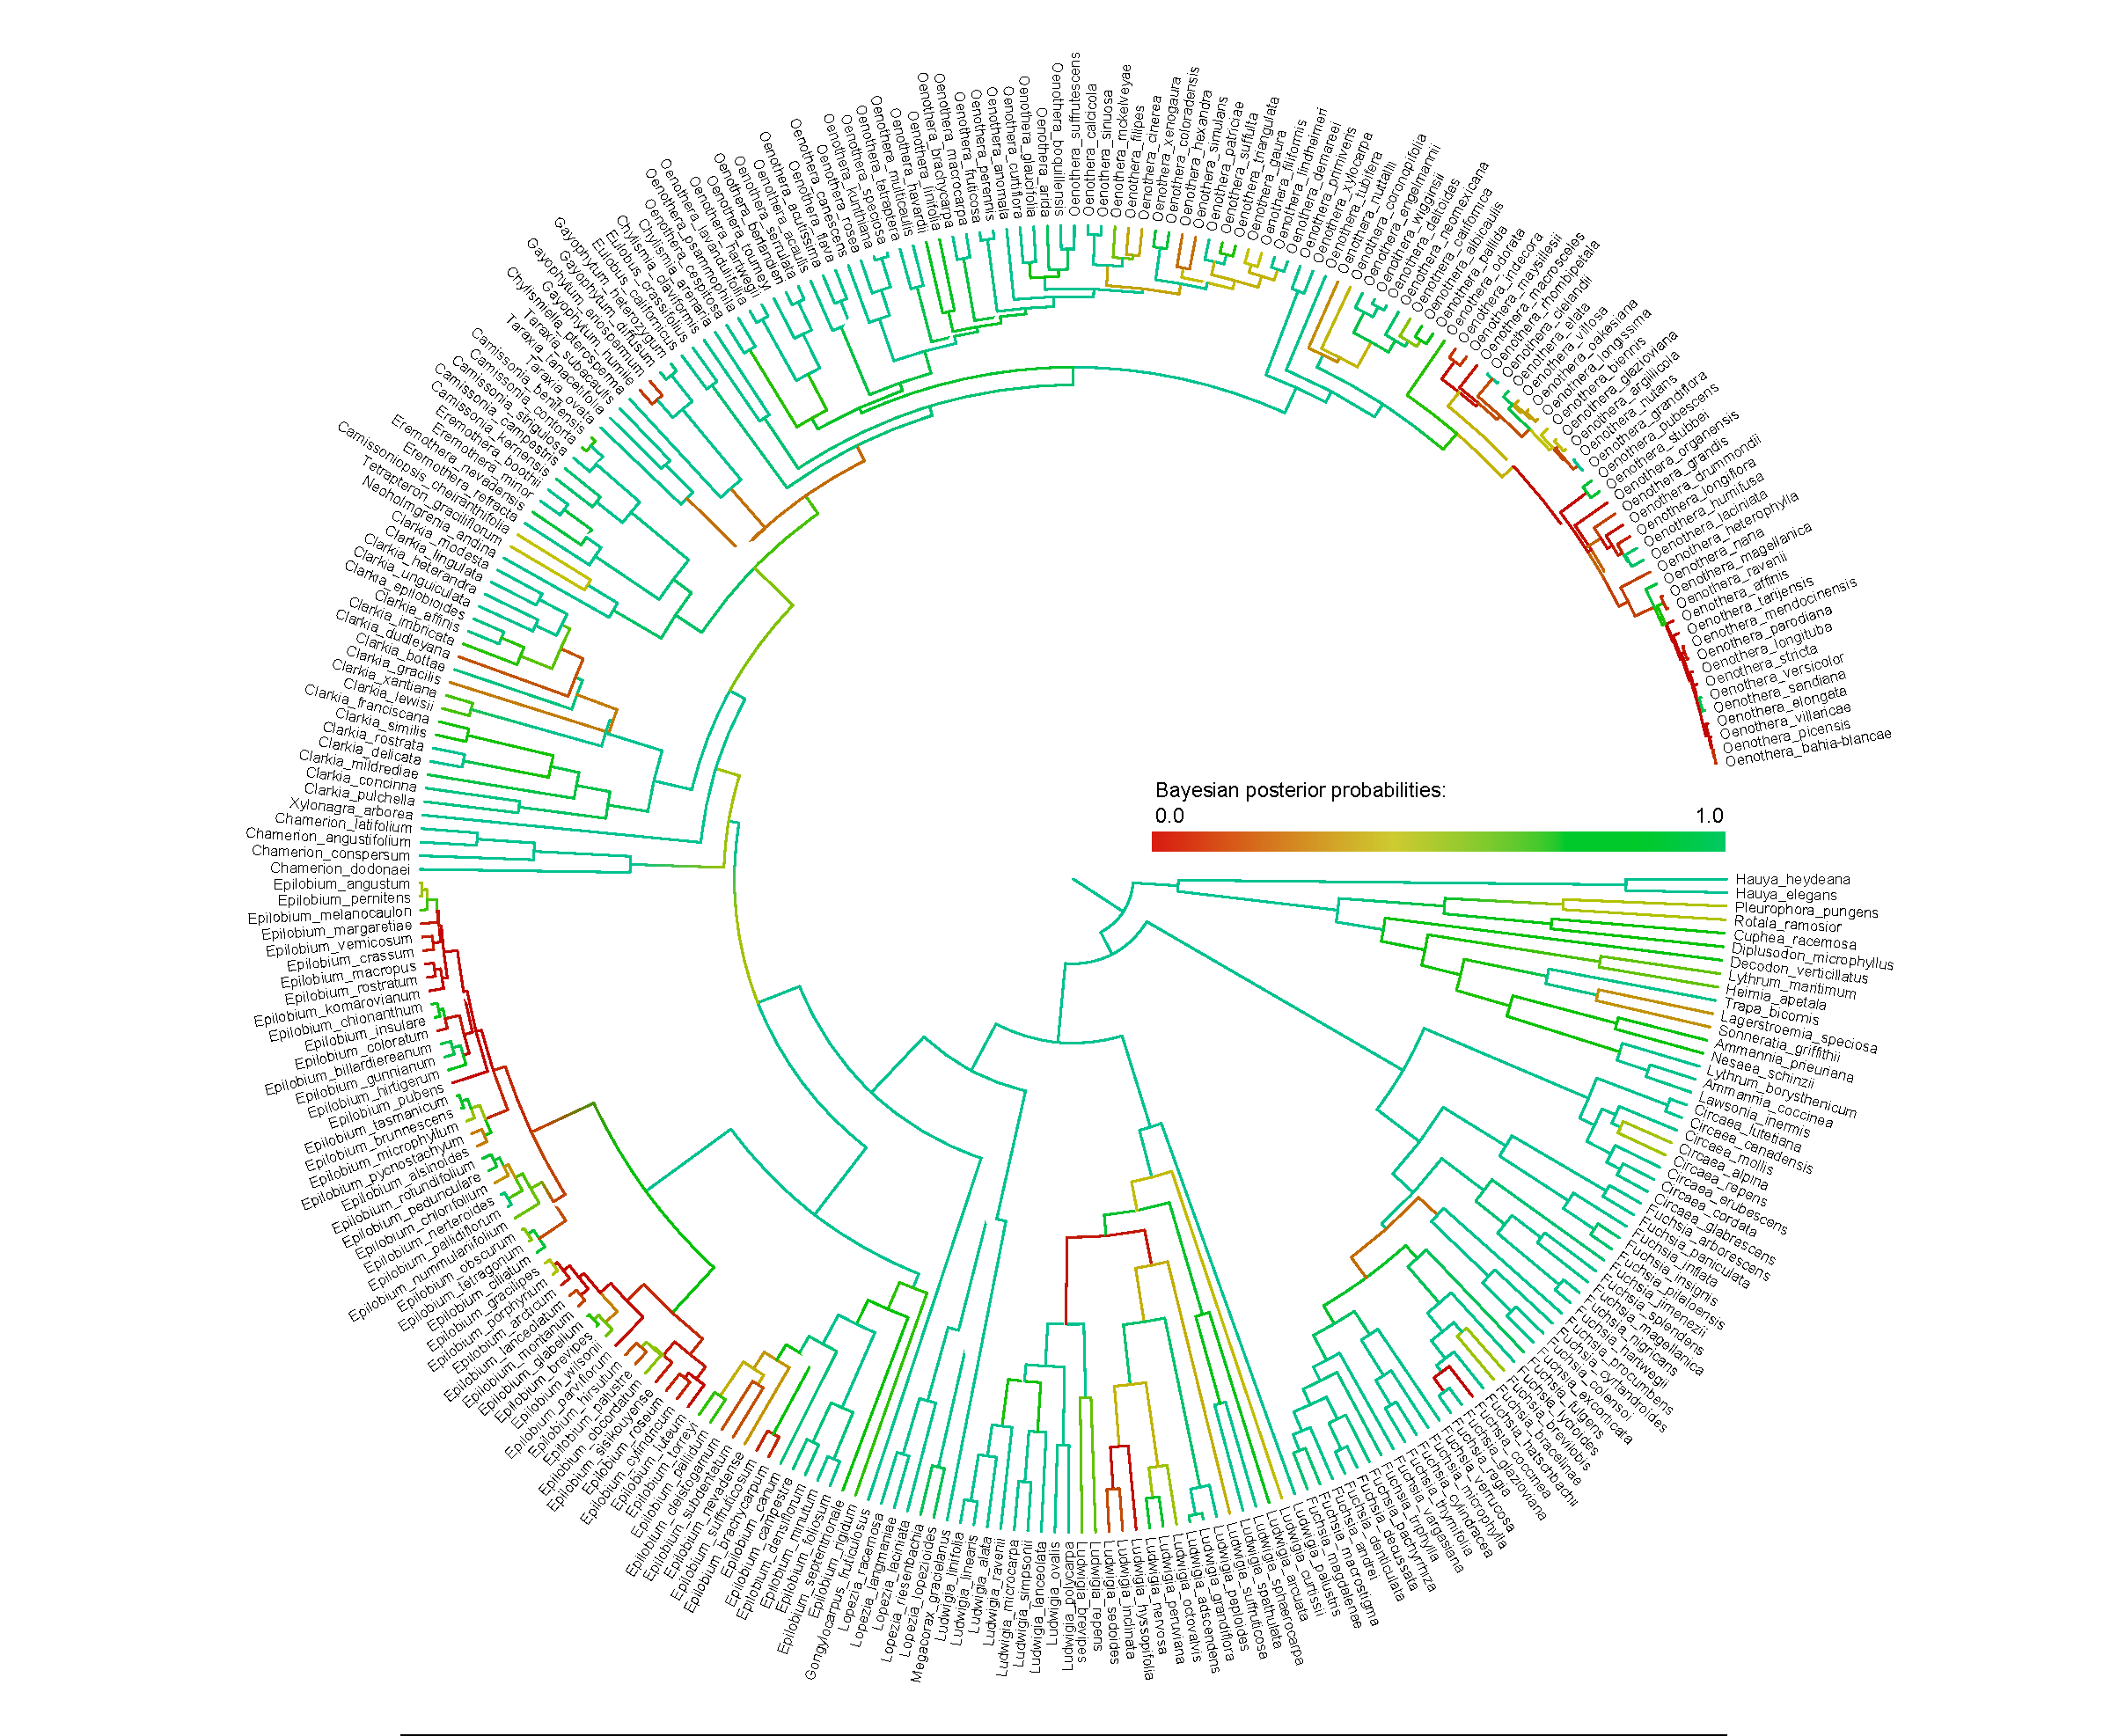
\includegraphics[width=1.6\linewidth, trim=0 10 0 0, clip=true]{colored_posterior}
    }
    \caption{
       Bayesian maximum clade credibility phylogeny of 280 Onagraceae taxa and 15 Lythraceae taxa. 
       Estimated posterior probabilities close to 1.0 are shown in green. All genera described in
       \citet{wagner2007revised} were found to be monophyletic with posterior probabilities of $> 0.95$
       except for sister genera \textit{Neoholmgrenia} and \textit{Camissoniopsis} (posterior = 0.31).
    }
    \label{posteriors}
\end{figure*}

\begin{figure*}[p]
    \vspace*{-2cm}
    \makebox[\linewidth]{
        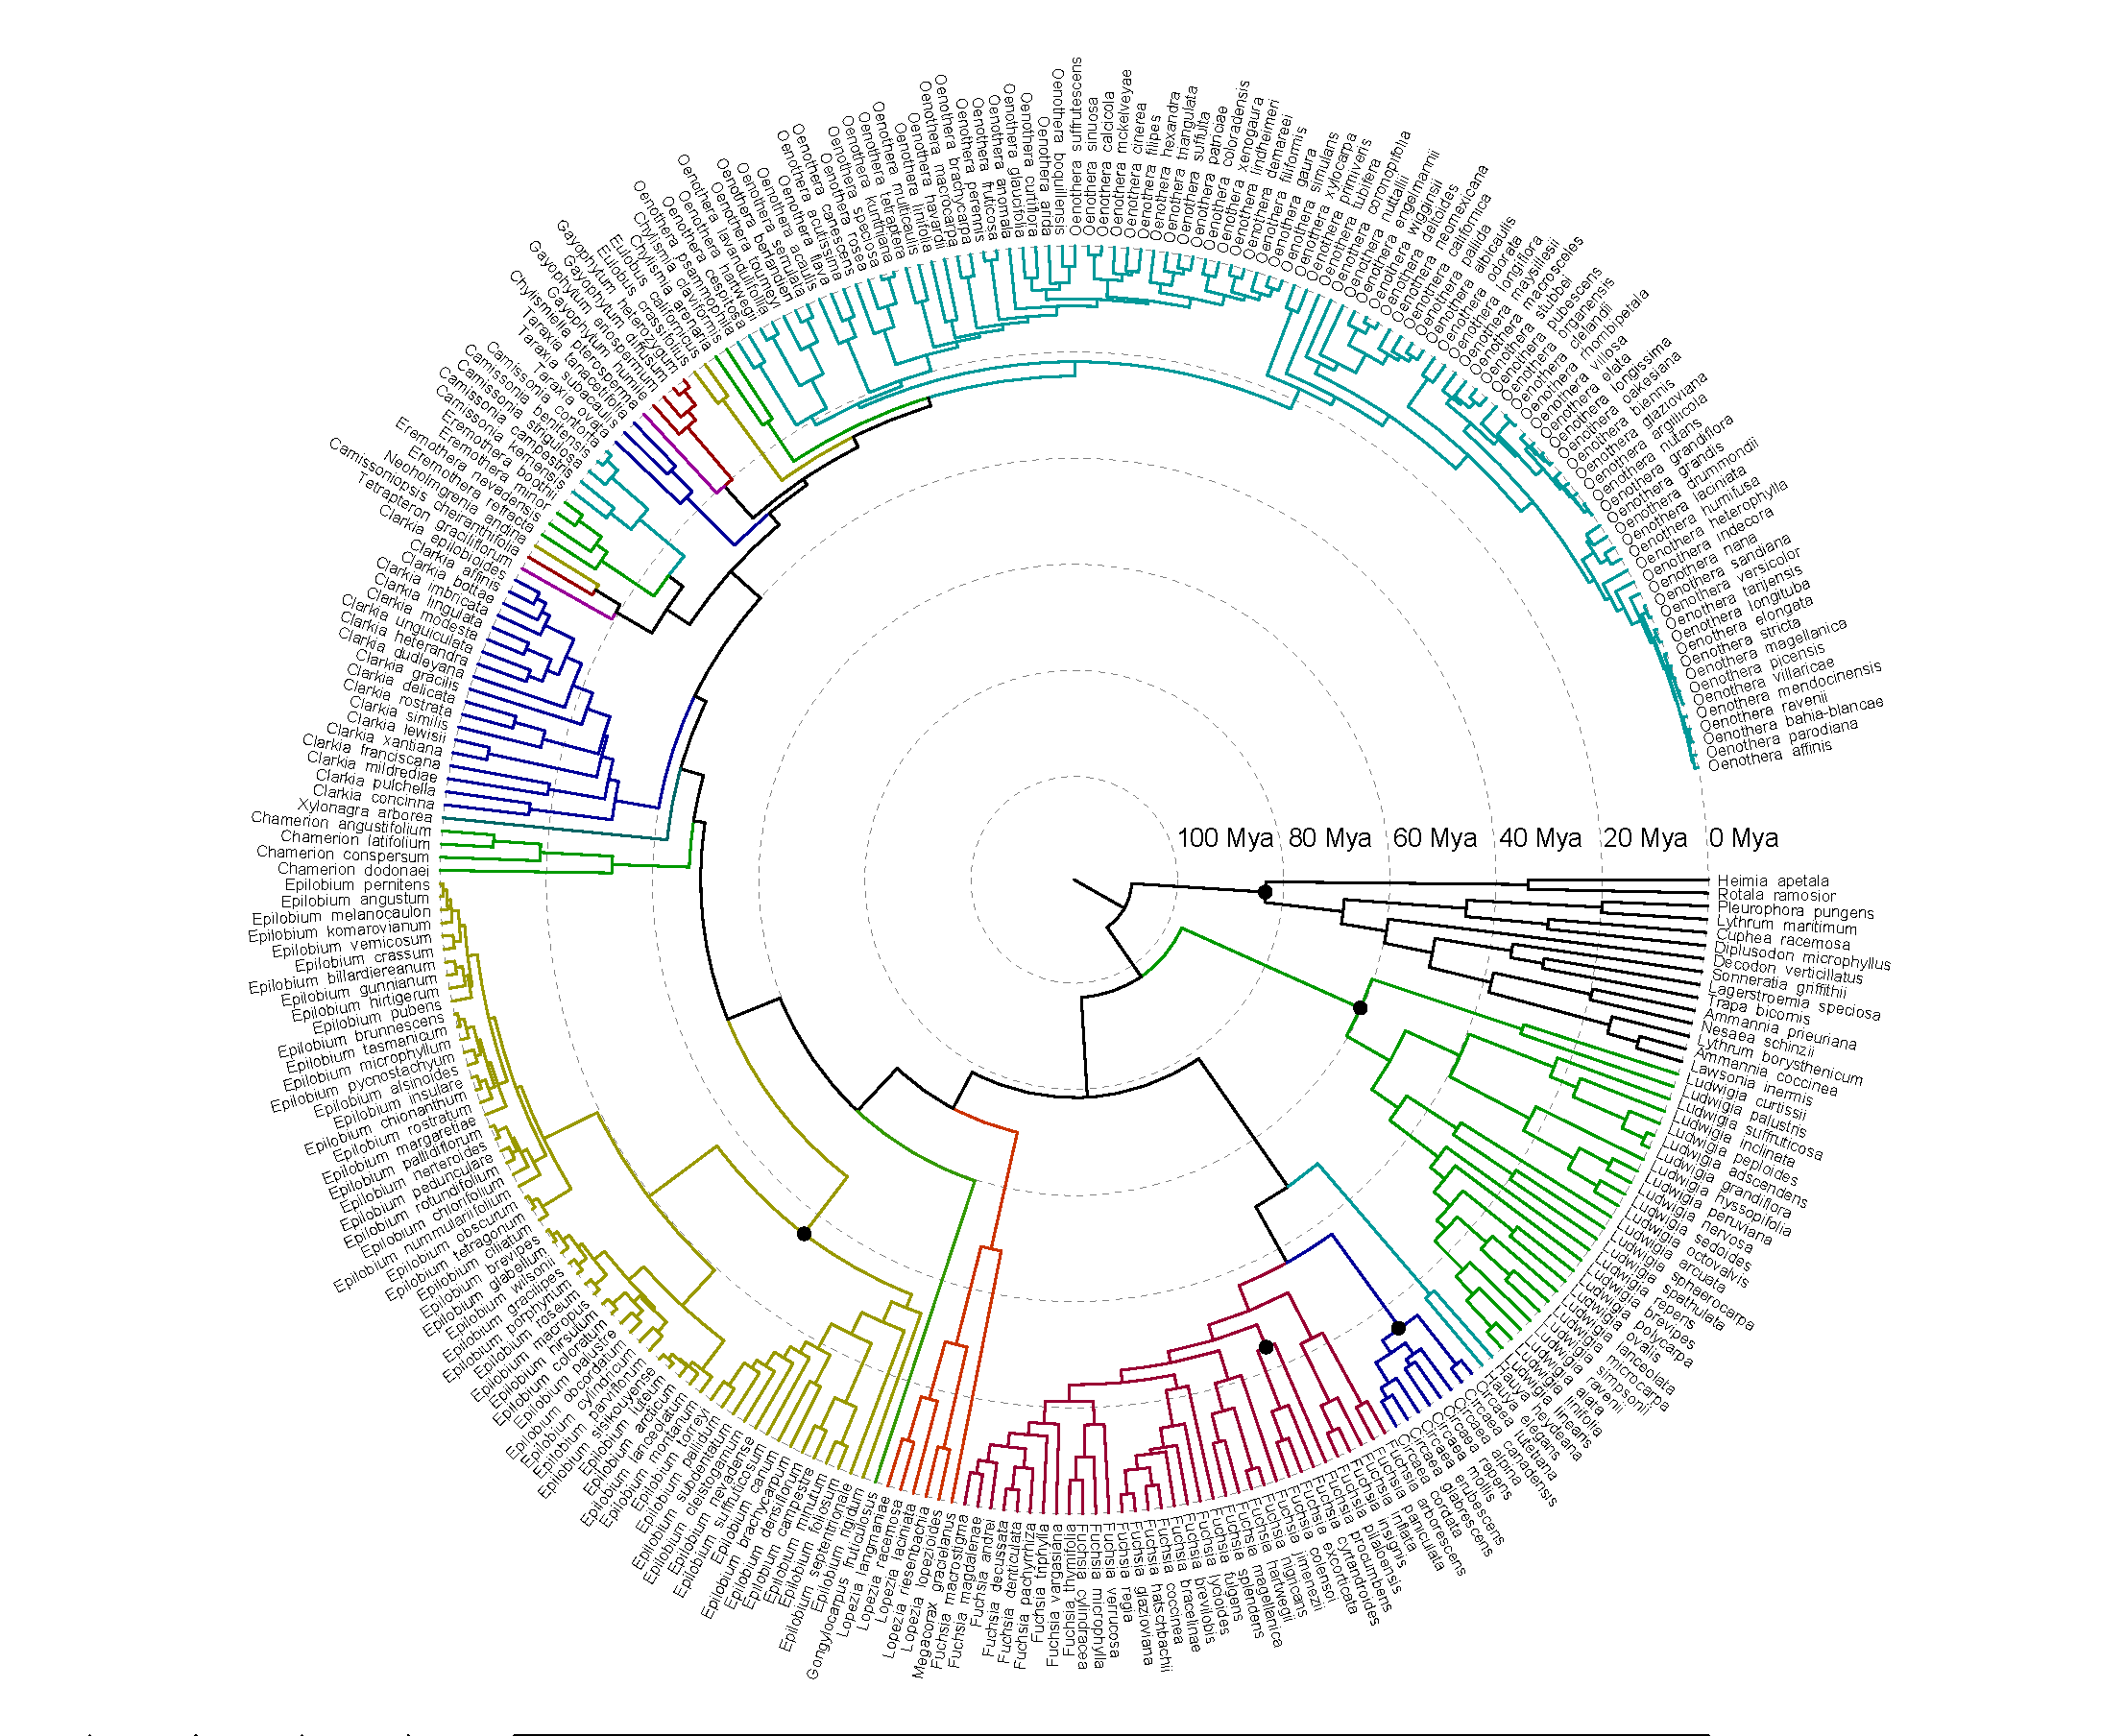
\includegraphics[width=1.6\linewidth, trim=0 10 0 0, clip=true]{time_colored_genera}
    }
    \caption{
       Bayesian chronogram of 280 Onagraceae taxa and 15 Lythraceae taxa.
       Approximate positions of fossil calibration points are shown as black circles.
       All genera described in \citet{wagner2007revised} are colored, and their
       divergence time estimates and \%95 HPD intervals can be seen in Table \ref{times}.
}
    \label{genera}
\end{figure*}


\begin{figure*}[p]
    \vspace*{-2cm}
    \makebox[\linewidth]{
        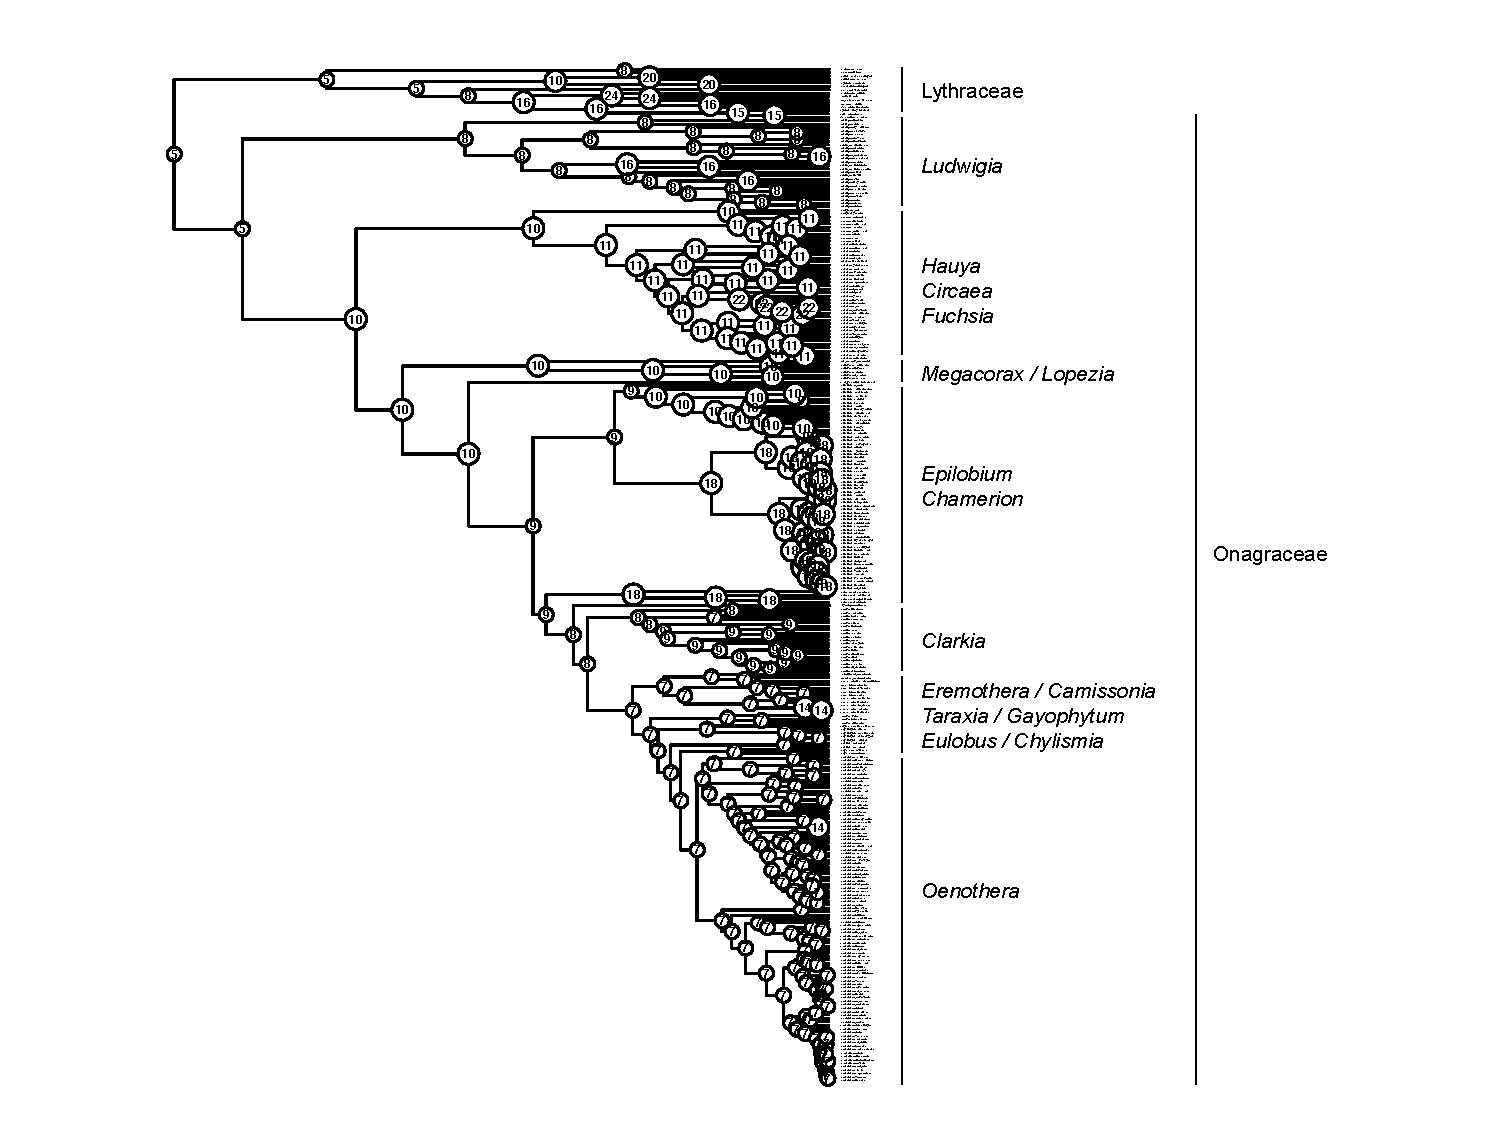
\includegraphics[width=1.6\linewidth, trim=0 0 0 0, clip=true]{chromtree_labeled}
    }
    \caption{
    Maximum likelihood estimates of ancestral chromosome numbers over the Bayesian MCC phylogeny
    using the 4 parameter ($\lambda$, $\delta$, $\mu$, $\rho$) model of chromosome evolution selected by Akaike's information criterion.
    The base number of Onagraceae is inferred to be $x=5$.
    }
    \label{chromtree}
\end{figure*}

\begin{figure*}[p]
    \vspace*{-2cm}
    \makebox[\linewidth]{
        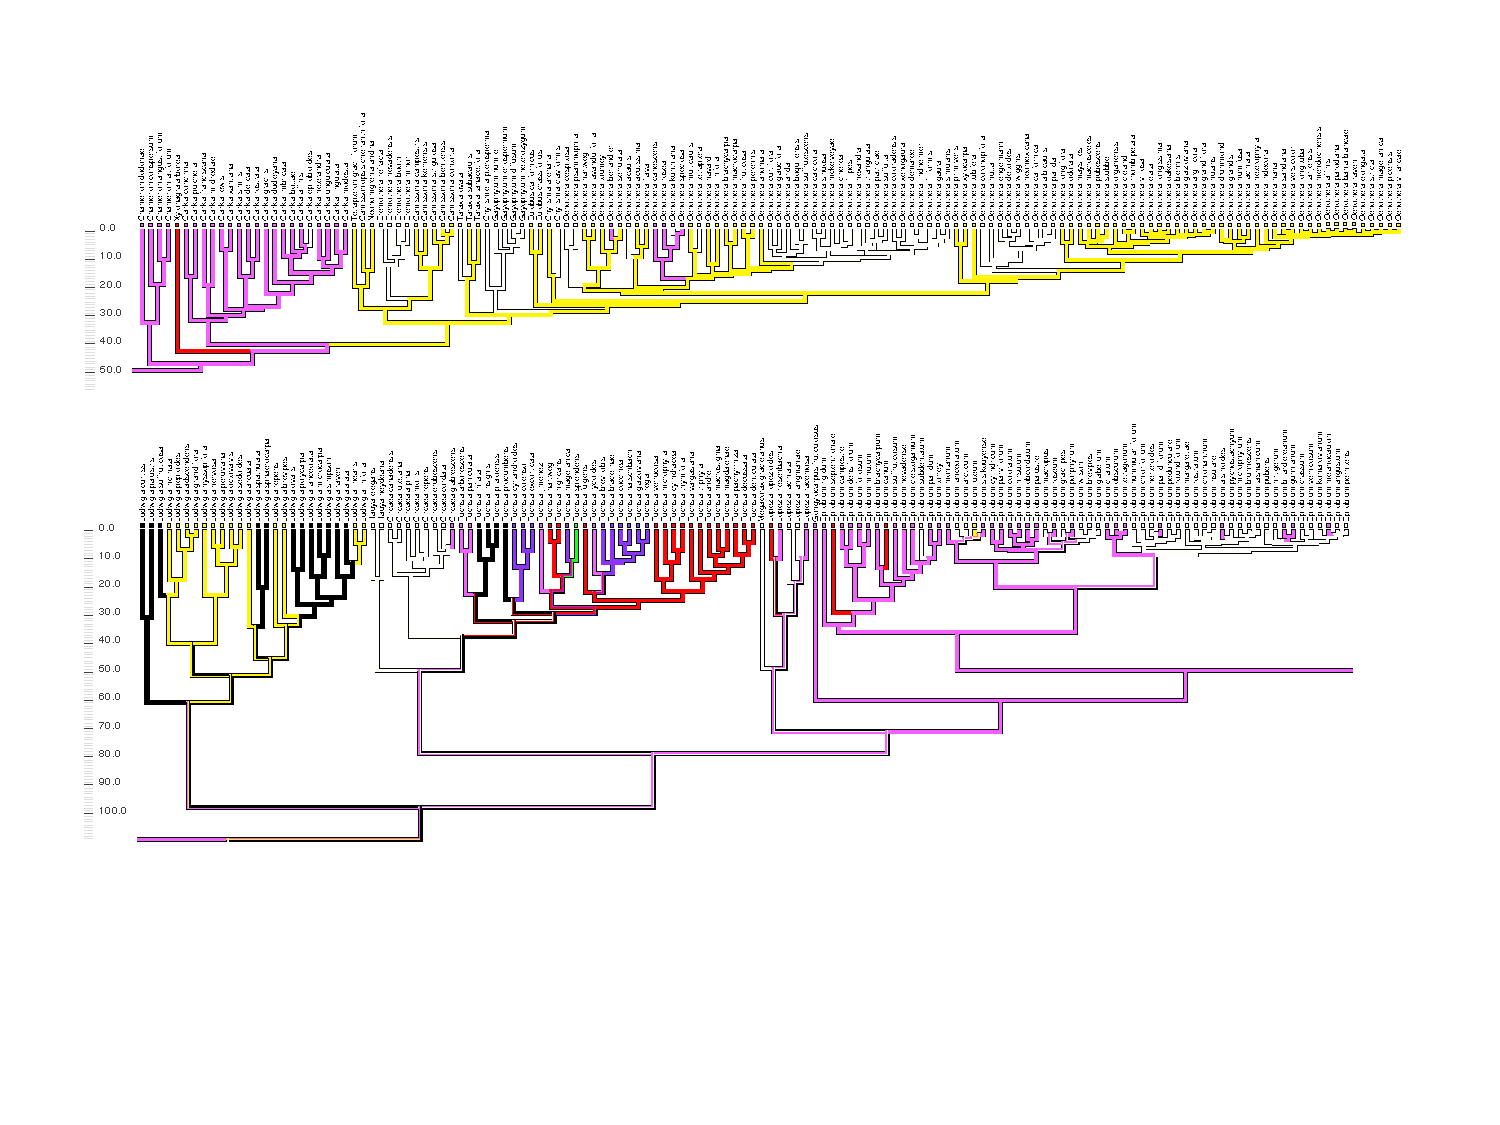
\includegraphics[width=1.6\linewidth, trim=0 0 0 0, clip=true]{petal_color}
    }
    \caption{
      Maximum likelihood ancestral state reconstruction of petal color.
      Black represents absence of petals. Vertical time scale is in millions of years before present.
    }
    \label{petal_color}
\end{figure*}

\begin{figure*}[p]
    \vspace*{-2cm}
    \makebox[\linewidth]{
        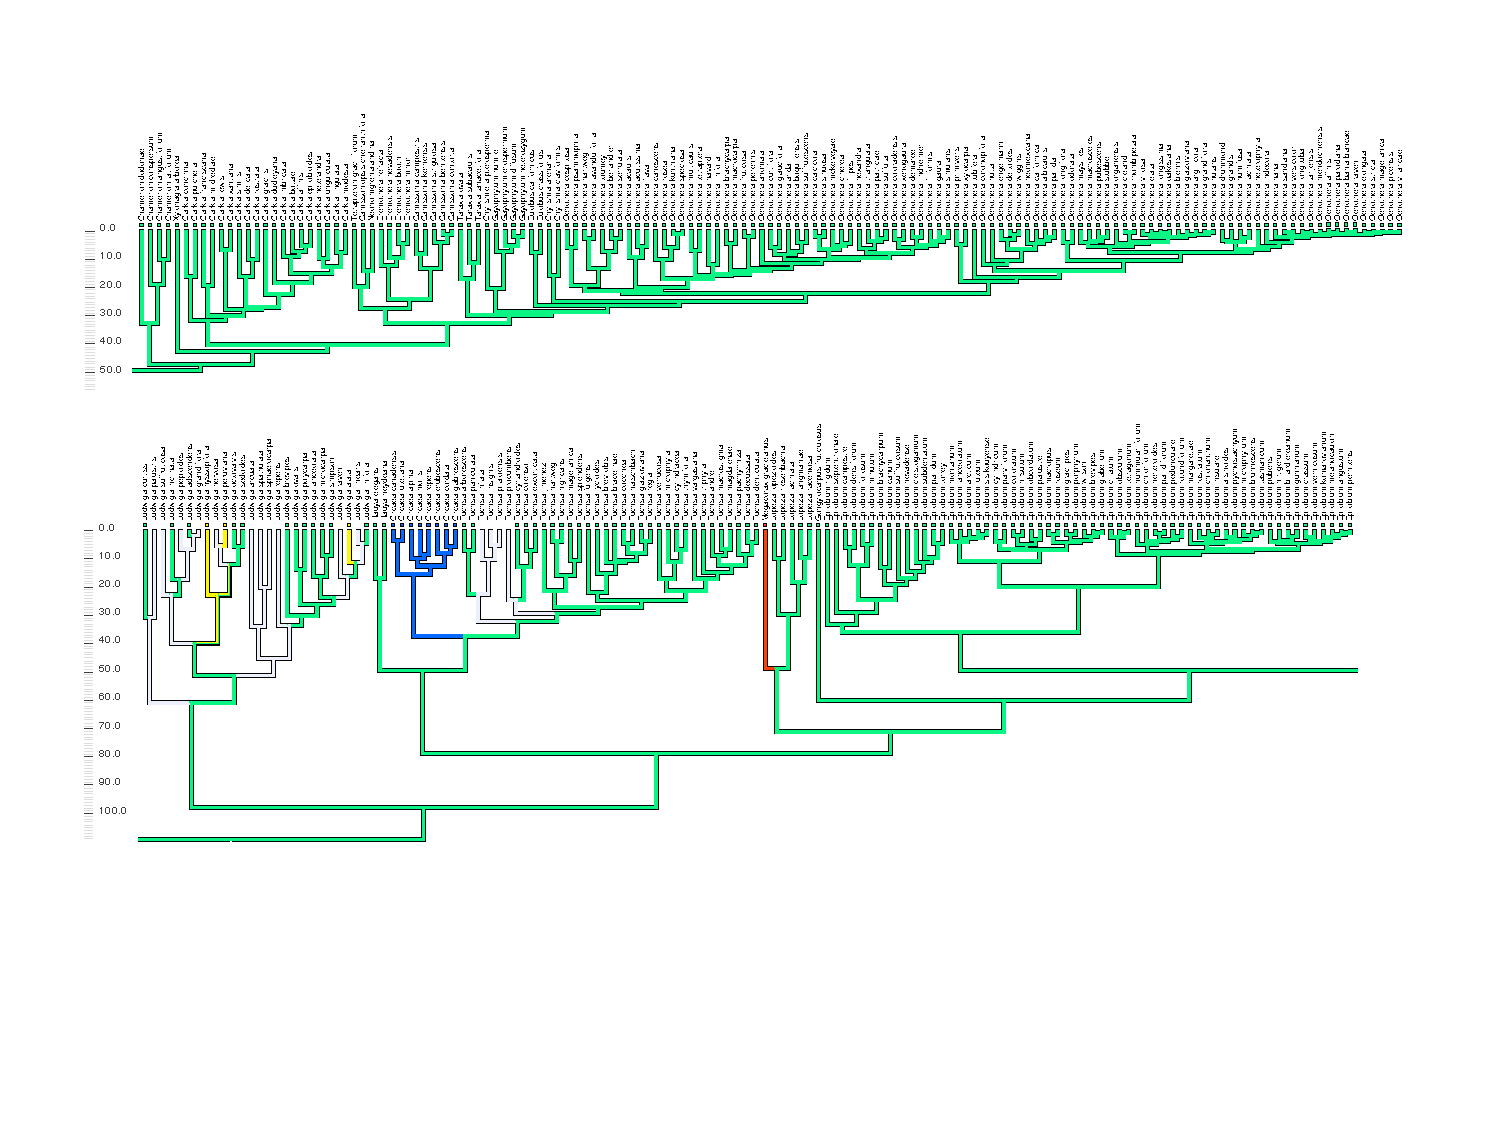
\includegraphics[width=1.6\linewidth, trim=0 0 0 0, clip=true]{petal_number}
    }
    \caption{
    Maximum likelihood ancestral state reconstructions of petal number. 
    White = 0, Blue = 2, Green = 4, Orange = 5. Vertical time scale is in millions of years before present.
    }
    \label{petal_number}
\end{figure*}

%%%%%%%%%%%%%%%%%%%%%%%
%% discussion
%%%%%%%%%%%%%%%%%%%%%%%

\section{Discussion}

discuss monophyly of tribe Epilobieae, which was supported in 
maximum likelihood analysis but not supported in Bayesian MCC, could be due to
fossil constraints.....

%%%%%%%%%%%%%%%%%%%%%%%
%% references
%%%%%%%%%%%%%%%%%%%%%%%

\section*{References}

\bibliography{manuscriptbib}

\end{document}
